\documentclass[12pt, a4paper]{article}
\title{Progetto Comunicazioni Ottiche B}
\author{Paolo Tosi, Nicolò Valsesia}

\usepackage{geometry}
\geometry{right=15mm, left=15mm, top=15mm, bottom=15mm}
\usepackage{graphicx}
\graphicspath{{../images/}}
\setlength{\parindent}{0em}

\usepackage{wrapfig}

\usepackage{amsmath}

\usepackage{hyperref}
\hypersetup{
    colorlinks=true,
    linkcolor=black,
    urlcolor=blue,
    bookmarks=true,
}

\begin{document}
\maketitle
\tableofcontents
\newpage

\section{Introduzione}
\label{sec:1}

La comunicazione in fibra ottica utilizza impulsi luminosi per trasmettere l'infomazione da un punto all'altro, solitamente in un raggio compreso tra le poche decine e le migliaia di chilometri.

\vspace{5mm}
In alcuni casi le linee possono coprire distanze di diverse migliaia di chilometri come nel caso dell'infrastruttura di cavi sottomarini transoceanici.
\vspace{5mm}
\subsection{Il Mezzo Trasmissivo e lo Spettro}
\label{sub:}

% subsection  (end)
La frequenza dell'onda luminosa portante è generalmente intorno a 200 THz, per una lunghezza d'onda di 1550 nm ($10^{-9} m$). Questa parte della banda è la parte con minore attenuazione dello spettro della fibra di silice che è il mezzo sul quale viene trasmessa l'onda luminosa, con minimi effetti di distorsione di canale.

La lunghezza d'onda effettiva all'interno del mezzo trasmissivo dielettrico (considerato omogeneo e isotropo e con bassa attenuazione) è definita dall'indice di rifrazione del mezzo $\eta$ .\\ Per il vuoto si ha $\eta = 1$ mentre per la silice vetrosa si ha per le lunghezze d'onda d'interesse $\eta = 1.46$.

Si ha quindi $ \lambda _m = \frac{\lambda}{\eta} $.
 
\vspace{5mm}
\begin{center}
\begin{tabular}{cc}
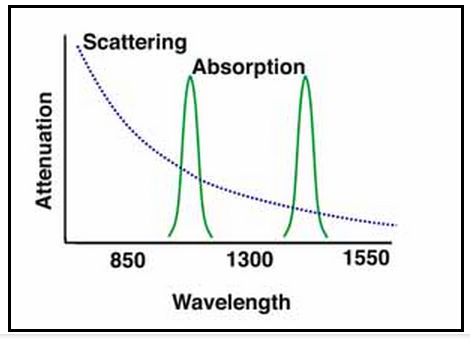
\includegraphics[scale = 0.4]{scattering.png}
&
\raisebox{5mm}{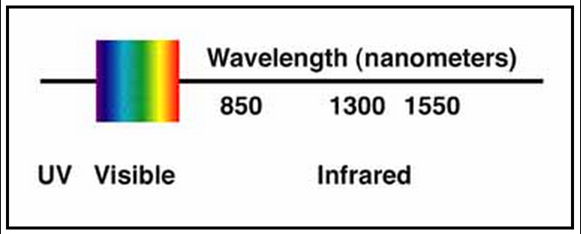
\includegraphics[scale = 0.4]{wavelenght.png}}
\end{tabular}
\end{center}
\vspace{5mm}

\subsection{Vantaggi}
\label{sub:vantaggi}

% subsection  (end)
Il bit-rate per l'informazione può raggiungere parecchie decine di $Gb/s$, attualmente la fibra Ethernet a $10Gb/s$ è lo standard industriale e $100Gb/s$ sarà introdotto nelle reti di fibra ottica globali.\\
Rispetto ad altri tipi di comunicazione la fibra ottica presenta due aspetti vantaggiosi:
\begin{itemize}
	\item Elevata frequenza delle portanti ottiche che permette di considerare bande di modulazione con larghezza $B$ molto elevata.
	\item La disponibilità di cavi in fibra ottica per trasmettere segnali a bassissima attenuuazione.
	(minima attenuazione $= 0.2 \frac{dB}{Km}$).\\
	Si trasmette con frequeze nell'intorno dell'infrarosso al di fuori degli intervalli d'assorbimento detti \textit{watering bands}.
\end{itemize}

\newpage
\subsection{L'onda portante}
\label{sub:}

\vspace{5mm}
L'onda luminosa portante può essere modulata secondo la modulazioni di ampiezza (ASK Amplitude Shift Keying), fase (PSK Phase Shift Keying) e frequenza (FSK frequency Shift Keying).\\
Nel nostro caso utilizziamo una ASK ON-OFF Non-Return-to-Zero.\\
Il segnale ottico trasmesso è definito dall'equazione:
\begin{equation}
	u(t) = \sqrt{2}a(t)\cos{[2\pi f_ct + \phi(t)]}
\end{equation}
con $f_c$ frequenza della portante.

Il segnale considerato è un segnale a banda stretta con banda \textit{B} tale che $B \ll f_c$.

Ciò ci consente di definire la rappresentazione complessa equivalente del segnale in banda base:
\begin{equation}
	\tilde{u}(t) = a(t)e^{i\phi(t)}
\end{equation}\
e dell'onda portante, defnita come:
\begin{equation}
	\tilde{c}(t) = \cos{(2\pi f_ct )}+ i\sin{(2\pi f_ct)} = e^{i2\pi f_c t}
\end{equation}

Per la ricezione del segnale si considera la potenza ottica ricevuta a valle del canale di trasmissione.
Questa è definita dal modulo quadro dell'inviluppo complesso:
\begin{equation}
	p(t) = |\tilde{u}(t)|^2 = a^2(t)
\end{equation}


\subsection{Canale di trasmissione}
\label{sub:Canale}

La risposta del canale è definita dalle caratteristiche del mezzo trasmissivo, in questo caso fibra di silice.
Per basse potenze ottiche (pochi mW) il suo comportamento è assimilabile a quello di un filtro lineare avente una funzione di trasferimento del tipo:
\begin{equation}
	H(f) = A(f) e^{j\beta(f)}
\end{equation}
dove:\begin{itemize}
	\item $A(f)$ è la risposta in ampiezza.
	\item $\beta(f)$ è la risposta in fase.
\end{itemize}

il segnale ottico all'uscita del canale è:
\begin{equation}
	u_{out}(t) = h(t) \ast u_{in}(t)
\end{equation}
Dato dalla convoluzione tra il segnale d'ingresso e la risposta impulsiva del canale.

Passando nel dominio della frequenza è possibile scrivere:
\begin{align*}
	U_{out}(f) &= H(f)U_{in}(f)\\
	H(f) &= \frac{U_{out}(f)}{U_{in}(f)}\\
\end{align*}

Il canale di trasmissione ha quindi l'effetto di moltiplicare l'ampiezza della componente spettrale per il termine $A(f)$ e di aggiungere alla fase della componente spettrale il termine $\beta(f)$.\\
Questi due termini rappresentano rispettivamente:
\begin{itemize}
	\item Coefficente di Trasmissione in Ampiezza
	\item Sfasamento del canale
\end{itemize}

per la poteza considero $A^2(f)$ detto \textit{coefficente di trasmissione in intensità} del canale. 

% subsection  (end)

\newpage
\subsection{Attenuazione}
\label{sub:attenuazione}

La perdita di potenza ottica costituisce uno dei fattori limitanti per il dimensionamento di linee di trasmissione in fibra ottica, in quanto riduce la potenza media del segnale ottico alla ricezione.

Le perdite sono condizionate da tre principali fattori:
\begin{enumerate}
	\item Perdita intrinseca data dalle caratteristiche fisiche del mezzo e scattering di Rayleigh.
	
	
	
	\item Perdite dovute al \textit{microbending}.
	\item Perdite dovute allo \textit{splicing} (connessione cavi in serie).
\end{enumerate}

La perdita intrinseca consiste principalmente nell'assorbimento dovuto alle impurità di OH presenti nel mezzo (dovuti all'umidità inglobata nella matrice vetrosa). É una funzione di $\lambda^{-6}$, più lunga la lunghezza d'onda minore è la perdita.\\
Lo scattering  (cambiamento della direzione della radiazione) è dato dalla struttura molecolare disordinata del vetro ed è direttamente proporzionale a $\lambda^{-4}$.

Per il silicio si hanno tre finestre "ottime" per la trasmissione, la prima a 800 nm presenta attenuazione $\alpha = 1.5$ dB/Km, quelle usate più frequentemente sono le due a 1300 e 1550 nm, con tolleranze di 80 e 40 nm rispettivamente.
in queste ultime fasce si hanno coefficenti di attenuazione più bassi $\alpha = 0.35$ dB/km e $\alpha = 0.2 $ dB/km.


\begin{figure}[h!]
\centering
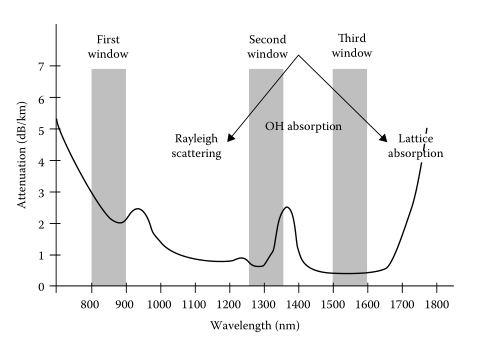
\includegraphics[scale=0.7]{attenuazione.png}
\caption{Attenuazione nel silicio in funzione della lunghezza d'onda}
\end{figure}

Le piegature della fibra cambiano l'angolo di incidenza tra il fronte d'onda e il confine nucleo-matello. Oltre un certo raggio di curvatura può venire a mancare l'angolo d'incidenza minimo per avere riflessione totale.
Nel \textit{microbending} le perdite sono causate da imperfezioni sul fronte nucleo-mantello formatesi durante la produzione della fibra.

\vspace{5mm}
Durante lo splicing due parti di fibra sono unite tra loro fondendo le estremità. Se queste non sono state tagliate e allineate correttamente prima della fusione si possono verificare disturbi alla trasmissione del segnale.\\
Offset dell'alineamento del valore di $1\mu m$ possono produrre perdite significative. Il disturbo è quindi una fuzione della distanza tra gli assi dei cavi connessi.

\begin{figure}[h!]
\centering
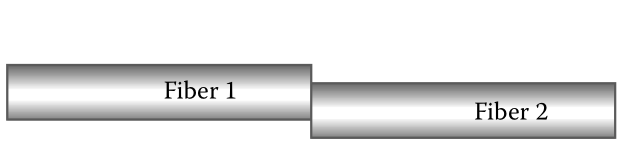
\includegraphics[scale=0.4]{splicing.png}
\caption{disallineamento in due fibre ottiche}
\end{figure}

Ogni componente spettrale alla generica frequenza $f$ verrà attenuata con trasmittività in potenza come:
\begin{equation}
	\frac{|U_{out}(f)|^2}{|U_{in}(f)|^2} = |H(f)|^2 = A^2(f)
\end{equation}

La risposta è una funzione esponenziale decrescente secondo la lunghezza L:
\begin{equation}
	A^2(f) = e^{-\alpha(f)L}  \rightarrow A(f) = e^{-\frac{1}{2}\alpha(f)L}
\end{equation}

$\alpha(f)$ è il \textbf{coefficiente d'attenuazione in potenza} in $[\frac{1}{m}]  o [\frac{1}{Km}]$  (è preferibile la notazione in decibel), $A(f)$ risposta in ampiezza del canale.


Si definisce l'\textbf{Attenuazione} come l'inverso del coefficiente di trasmissione:
\begin{equation}\label{Q_eq}
	Q(f) = \frac{1}{A^2(f)} = e^{\alpha(f)L}
\end{equation}
Per la trasmissione considerata nel progetto con $\lambda = 1550 nm$ si considera $\alpha = 0.2 $ dB/Km.

Risulta essere:
\begin{equation}
	\alpha = \frac{0.2}{4.343} Km^{-1} = 0.046 Km^{-1} = 4.6*10^{-5} m^{-1}
\end{equation}

% subsection  (end)

\vspace{10mm}
\subsection{Dispersione Cromatica}
\label{sub:dispersione}

La dispersione cromatica è dovuta al fatto che in fibra, frequenze diverse si propagano a velocità diverse. La principale causa è la dipendenza dell’indice di rifrazione dalla frequenza dell'onda.

L'effetto della dispersione è tanto più grande quanto è più largo lo spettro del segnale trasmesso.

\vspace{5mm}
La risposta in fase nell'intorno di $f_c$ può essere approssimata con lo sviluppo in serie di Taylor del secondo ordine:

\begin{equation}
	\beta(f) \cong \beta(f_c) + \frac{d\beta(f_c)}{df}(f-f_c) + \frac{1}{2}\frac{d^2\beta(f_c)}{df^2}(f-f_c)^2
\end{equation}

Esplicitando  la dipendenza di $\beta(f)$ dalla lunghezza L del tratto di fibra ottengo tre parametri $\beta_0 , \beta_1, \beta_2$.

\begin{equation}
	\beta(f) \cong \beta_0(f_c)L + \beta_1(f_c)L*(f-f_c) + \frac{1}{2}\beta_2(f_c)L*(f-f_c)^2
\end{equation}

\begin{enumerate}
	\item Il termine di ordine 0 esprime la risposta in fase della portante:
	\begin{equation}
		\beta(f_c) = \beta_0(f_c)L
	\end{equation}
	
	È un'approssimazione della risposta in fase come una retta $\beta_0*L$
	
	Nella simulazione si considera $\beta_0$ costante uguale per tutte le frequenze. Poichè del segnale equivalente in banda base si considera solamente l'inviluppo, tale offset non influisce sul calcolo della risposta in fase del filtro di canale.
	
	Il ritardo di fase $\tau_p$ è il ritardo temporale (sec) della portante, uguale al numero di cicli della portante per la durata temporale di un suo ciclo.
	
	
	\begin{equation}
		\tau_p = \frac{\beta(f_c)}{2\pi f_c} = \frac{\beta_0(f_c)
		*L}{2\pi f_c}
	\end{equation}

	\item Il termine di ordine 1 contiene la derivata della risposta in frequenza valutata alla portante ed è legato al ritardo di gruppo $\tau_G$
	
	\begin{equation}
		\tau_G = \frac{\beta_1(f_c)*L}{2\pi}
	\end{equation}

		Il ritardo di gruppo indica il ritardo con cui l'energia dei segnali arriva al ricevitore, anch'esso non influisce sul calcolo delle prestazioni in quanto si considera che al ricevitore sia stato introdotto un meccanismo di recupero del sincronismo. 

	\item Il termine di ordine 2 è la derivata seconda della risposta in fase dle canale, è un indice della distorsione (espansione o compressione) dell'intervallo di trasmissione del bit.
	
	L'effetto di questo termine può essere compensato introducendo un tratto di canale detto \textit{Modulo di compensazione} realizzato con fibra speciale avente coeficiente di dispersione cromatica $D = -100\frac{\rho\text{s}}{\text{nm*Km}}$.
	
	Questa presenta un  che compensa la dispersione cromatica del canale, ma rappresenta un'ulteriore fonte di attenuazione del segnale.
	
	Considerando l'utilizzo di 1Km di fibra speciale ogni 6Km di fibra standard permette di considerare nulla la risposta in fase del canale, a patto di introdurre un ulteriore termine d'attenuazione in potenza con coefficiente:
	\begin{equation}
		\alpha_{comp} = 0,5 \hspace{0.2cm} \text{dB/Km}
	\end{equation} 
		
\end{enumerate}

% subsection dispersione (end)

\subsection{Ricevitore a Rivelazione Diretta}
\label{sub:rice}


Il segnale giunto in fase di ricezione sarà caratterizzato dalla componente $a(t)$ (segnale dopo il filtro formatore)  la quale viene atenuata secondo $Q(f)$ (eq. \ref{Q_eq}) e subisce un ritardo di fase per l'effetto del filtro di canale $h_c(t)$.

\begin{equation}
	\tilde{u}_R(t) = a_R(t)e^{i\phi_r(t)}
\end{equation}

L'implementazioen dei ricevitori ottici dipende dal formato di modulazione del segnale: analogico o digitale, On-Off keying o a livelli multipli.

Nel progetto si è implementato un sistema DD-OOK (Direct Detection ON/OFF keying).
Un sistema di ricezione ottica digitale è costituito da:
\begin{itemize}
	\item Un \textbf{Fotodiodo}, il cui scopo è quello di convertire la potenza dell'onda luminosa [Watt] in corrente elettrica [Ampère], secondo un fattore detto \textit{responsivity} [A/W].
	La sua implementazione introduce rumore \textit{Shot}, prodotto dalle fluttuazioni casuali di natura quantistica della fotocorrente generata dal fotodiodo.\\
	Trattandosi di un rumore gaussiano bianco questo ha media nulla e deviazione standard:\\
	\begin{align*}
	\sigma_k^{shot} = \sqrt{2e\mu_kB_n}  \hspace{5mm}[A]
\end{align*}

	Dove $e = 1.6*10^{-19} $[C] è la carica elementare, $\mu_k$ è il valore medio del segnale elettrico corrispondente al bit k, $B_n =7.5 *10^9$[Hz] è la Banda equivalente di rumore.
	
	\item Un \textbf{TIA} Amplificatore a Transimpedenza, che converte la corrente a bassa intensità in una tensione [V], introducendo una componente di rumore \textit{Elettrico} determinata dal passaggio di corrente attraverso l'impedenza dell'amplificatore.
	In fase di progetto si è considerato il rumore equivalente in ingresso al TIA, gaussiano bianco con media nulla e deviazione standard:
	\begin{align*}
	\sigma_n^{termico} = NEC\sqrt{B_n} \hspace{5mm} [A]
\end{align*}

	Dove il Rumore Equivalente di Corrente NEC$=20 \hspace{1.5mm}[\frac{\rho A}{\sqrt{Hz}}]$  e $B_n = 7.5 *10^9$[Hz].
	
\end{itemize}

\vspace{5mm}
Nella progettazione del sistema è stato considerato solamente l'effetto del rumore equivalente in ingresso al TIA.

%INSERIRE GRAFICO QUI!

% subsection  (end)

\subsection{Campionamento e Decisore a soglia}
\label{sub:decisore}


Il segnale prima di essere campionato è nella forma:
\begin{align}
	r(t) = v(t) + n(t)
\end{align}
Dove $v(t)$ rappresenta la componente di segnale utie e $n(t)$ è la componente di ruumore introdotta dall'Amplificatore.

I valori da inviare al decisore sono ottenuti campionando il segnale ricevuto a istanti (Ts/2 + kTs) con k intero [0; N -1simboli]. In questo modo il valore è letto nel punto di massimo al centro di ciscun intervallo di simbolo.

\begin{align}
	r_k = r(kTs + \frac{Ts}{2}) = v(kTs + \frac{Ts}{2}) + n(kTs + \frac{Ts}{2})
\end{align}

I valori ottenuti dal campionamento sono confrontati con il valore della soglia $\lambda$, definita come il valor medio del segnale, calcolato al ricevitore.

L'errore di trasmissione viene quantificato con il parametro BER \textit{bit error rate}, ovvero: 
\begin{align*}
	\text{BER} =  \frac{\text{n° bit errati}}{\text{n° bit trasmessi}}
\end{align*}
%CHIEDERE PARERE

% subsection  (end)

%Section end

\newpage
\section{Implementazione e Codice Matlab}
\label{sec:2}

Il progetto è stato svolto attraverso il software \textbf{Matlab}.

\subsection{Definizione Parametri Principali}
\label{sub:2.1}

\begin{figure}[h!]
\centering
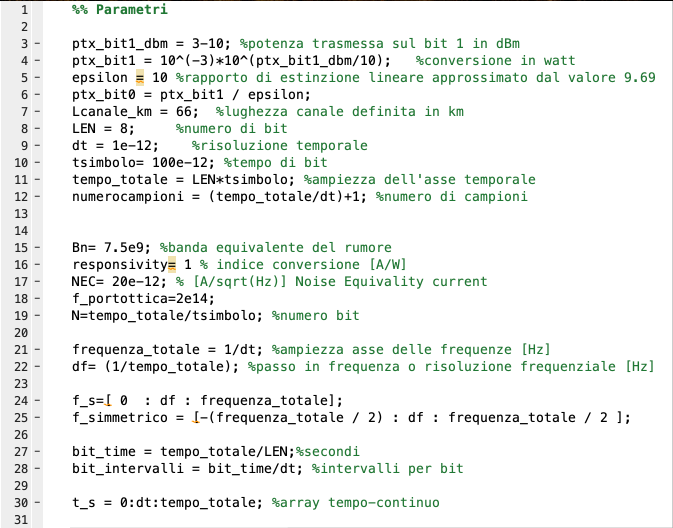
\includegraphics[scale=1.0]{parametri.png}
\caption{}
\label{}
\end{figure}

Variabili Principali:
\begin{itemize}
	\item Lcanale\_Km: la lunghezza del canale in Km. 
	%CHIEDERE PER PROB. ERRORE
	\item LEN: numero di bit trasmessi
\end{itemize}

Vettore Tempo t\_s: definto da un valore 0 a fino al valore \textit{tempo\_totale} ottenuto dalla moltiplicazione tra numero di bit \textit{LEN} e il tempo di simbolo \textit{tsimbolo} $= 100 \rho$s. Con passo \textit{dt} $= 1 \rho$s.

\vspace{5mm}
Vettore Frequenze f\_s: definto da un valore 0 a fino al valore \textit{frequenza\_totale} ottenuto dal rapporto 1/\textit{dt}.  Con passo \textit{df} $= 1/$\textit{tempo\_totale}.

% subsection  (end)

\newpage
\subsection{Generazione del Segnale}
\label{sub:2.2}

\begin{figure}[h!]
\centering
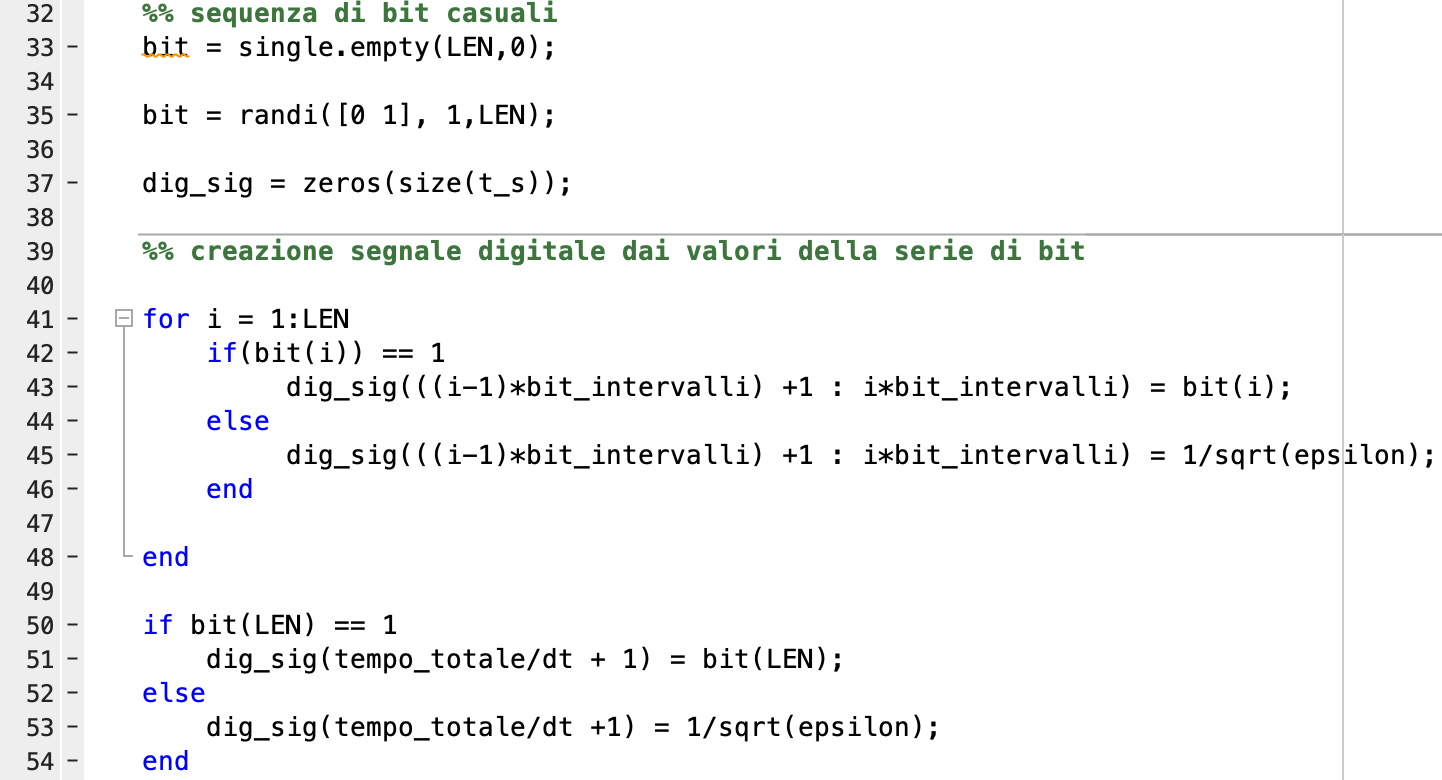
\includegraphics[scale=0.5]{sequenzabin.png}
\caption{}
\label{}
\end{figure}


La funzione \textit{randi} è utilizzata per generare un vettore di valori binari casuali di lunghezza \textit{LEN}.

Il primo ciclo For utilizza il vettore \textit{bit} per generare il segnale rettangolare con valori d'ampiezza 1 e 0 per i bit.

Per mantenere un rapporto d'estinzione lineare $\epsilon \cong 10$, il livello d'ampiezza 'basso' del bit 0 è stato posto a 1/3. (Figura \ref{dig_sig}).

  \begin{figure}[h!]
  \centering
  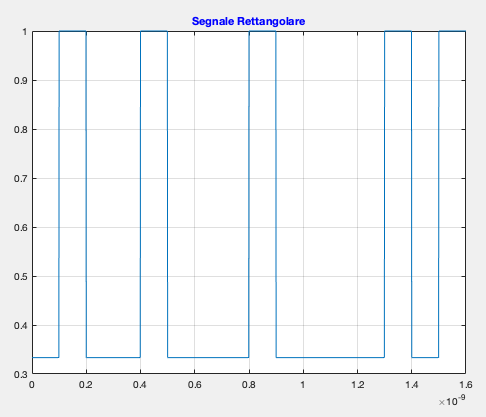
\includegraphics[scale = 0.6]{digsig.png}
  \caption{segnale digitale di 16 bit}
  \label{dig_sig}
  \end{figure}


\newpage
\begin{figure}[h!]
\centering
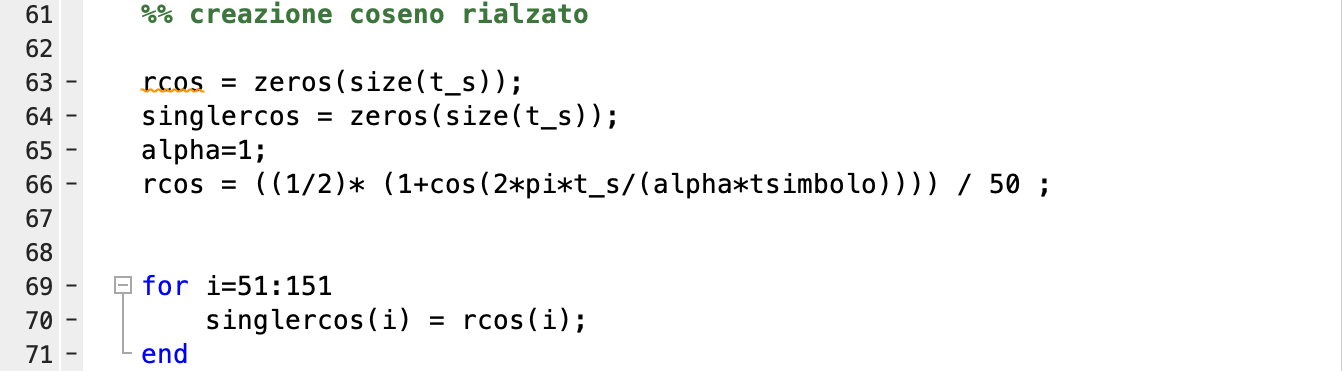
\includegraphics[scale=0.4]{cosenorialzato.png}
\caption{}
\label{6}
\end{figure}

Poichè il segnale rettangolare generato è un'idealizzazione, ovvero non fisicamente realizzabile, si è implementato un filtro a coseno rialzato centrato in Ts.

Questo ha lo scopo di rendere le transizioni del segnale sinusoidali e non istantanee. 
Il filtro è definito di \textit{Smoothing}.

\begin{figure}[h!]
\centering
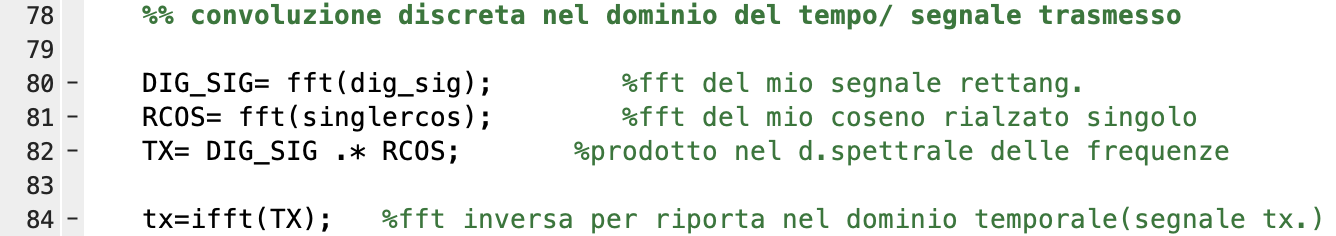
\includegraphics[scale=0.4]{convoluzionediscreta.png}
\caption{}
\label{}
\end{figure}

Attraverso l'uso della Fast Fourier Transform FFT si ottiene la risposta in frequenza del filtro, che moltiplicata per la trasformata del segnale digitale \textit{DIG\_SIG} definisce il segnale trasmesso \textit{TX} nel dominio della frequenza.

\vspace{5mm}
\begin{center}
\begin{tabular}{c c}
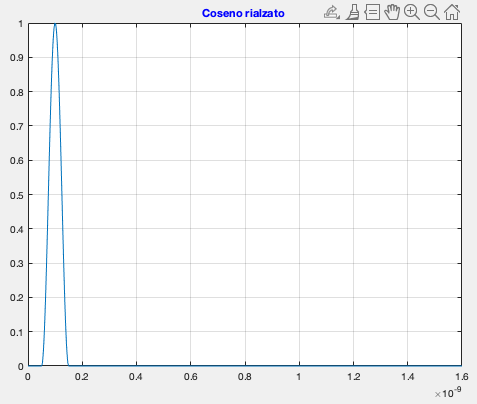
\includegraphics[scale = 0.7]{cosrialzatoimg.png}
&
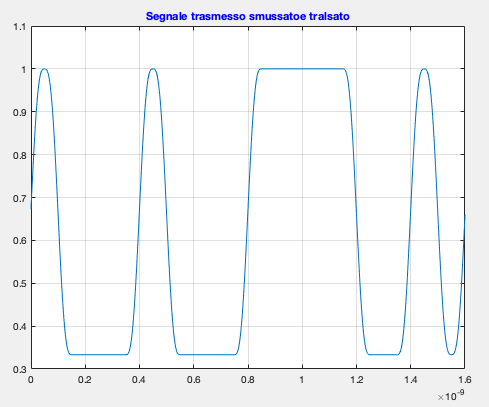
\includegraphics[scale = 0.7]{segnalesmussato.png}
\end{tabular}
\end{center}



% subsection  (end)

% section  (end)



\end{document}